\iffalse
\let\negmedspace\undefined
\let\negthickspace\undefined
\documentclass[journal,12pt,twocolumn]{IEEEtran}
\usepackage{cite}
\usepackage{amsmath,amssymb,amsfonts,amsthm}
\usepackage{algorithmic}
\usepackage{graphicx}
\usepackage{textcomp}
\usepackage{xcolor}
\usepackage{txfonts}
\usepackage{listings}
\usepackage{enumitem}
\usepackage{mathtools}
\usepackage{gensymb}
\usepackage{comment}
\usepackage[breaklinks=true]{hyperref}
\usepackage{tkz-euclide} 
\usepackage{listings}
\usepackage{gvv}
\def\inputGnumericTable{}                                 
\usepackage[latin1]{inputenc}                                
\usepackage{color}                                            
\usepackage{array}                                            
\usepackage{longtable}                                       
\usepackage{calc}                                             
\usepackage{multirow}                                         
\usepackage{hhline}                                           
\usepackage{ifthen}                                           
\usepackage{lscape}

\newtheorem{theorem}{Theorem}[section]
\newtheorem{problem}{Problem}
\newtheorem{proposition}{Proposition}[section]
\newtheorem{lemma}{Lemma}[section]
\newtheorem{corollary}[theorem]{Corollary}
\newtheorem{example}{Example}[section]
\newtheorem{definition}[problem]{Definition}
\newcommand{\BEQA}{\begin{eqnarray}}
\newcommand{\EEQA}{\end{eqnarray}}
\newcommand{\define}{\stackrel{\triangle}{=}}
\theoremstyle{remark}
\newtheorem{rem}{Remark}

\begin{document}

\bibliographystyle{IEEEtran}
\vspace{3cm}

\title{GATE IN21 44}
\author{EE23BTECH11043 - BHUVANESH SUNIL NEHETE$^{*}$% <-this % stops a space
}
\maketitle
\newpage
\bigskip

\renewcommand{\thefigure}{\theenumi}
\renewcommand{\thetable}{\theenumi}

\bibliographystyle{IEEEtran}

\textbf{Question:}
The input signal shown below \\
\input{2021/IN/44/figs/xn}\\
is passed through the filter with following taps\\
\input{2021/IN/44/figs/n}\\
The number of non-zero output samples is \underline{\hspace{1cm}}.\\

\solution
\fi
\begin{align}
    h\sbrak{n}=-\delta\sbrak{n}+2\delta\sbrak{n+1}-\delta\sbrak{n+2}
\end{align}
\begin{align}
    y\sbrak{n}&=x\sbrak{n}*h\sbrak{n}\\
    &=x\sbrak{n}*\brak{-\delta\sbrak{n}+2\delta\sbrak{n+1}-\delta\sbrak{n+2}}\\
    y\sbrak{n}&=-x\sbrak{n}+2x\sbrak{n+1}-x\sbrak{n+2}
\end{align}

\input{2021/IN/44/figs/yn}
The number of non-zero output samples is $10$.

\begin{figure}
    \centering
    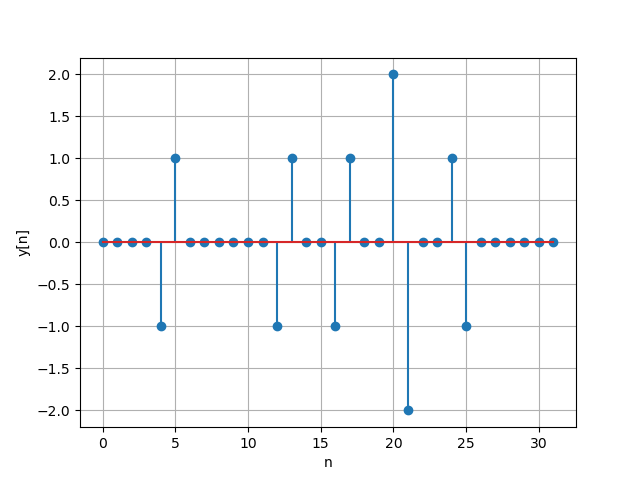
\includegraphics[width=1\linewidth]{2021/IN/44/figs/fig.png}
\end{figure}
